\documentclass{article}
\usepackage{graphicx}
\graphicspath{ {./images/} }
\title{Monopoly Math \\ \large The mathematics behind the game of Monopoly }
\author{Lars Kwant}

\begin{document}

\maketitle

\tableofcontents

\newpage

\section{Introduction to the game}
\subsection{Goal of the game}
Monopoly is a game played by 2 to 6 individuals. The goal of the game is to become the player that does not go bankrupt. The goal of each individual is therefore to make as much money as possible in order to make each opponent go bankrupt. The player does this by buying property and issuing rent on opponents if they land on one of these properties.\\

\subsection{The board}
The board is seperated into 40 squares. Each square has its own unique action attached to it. 
\begin{figure}[h]
\centering
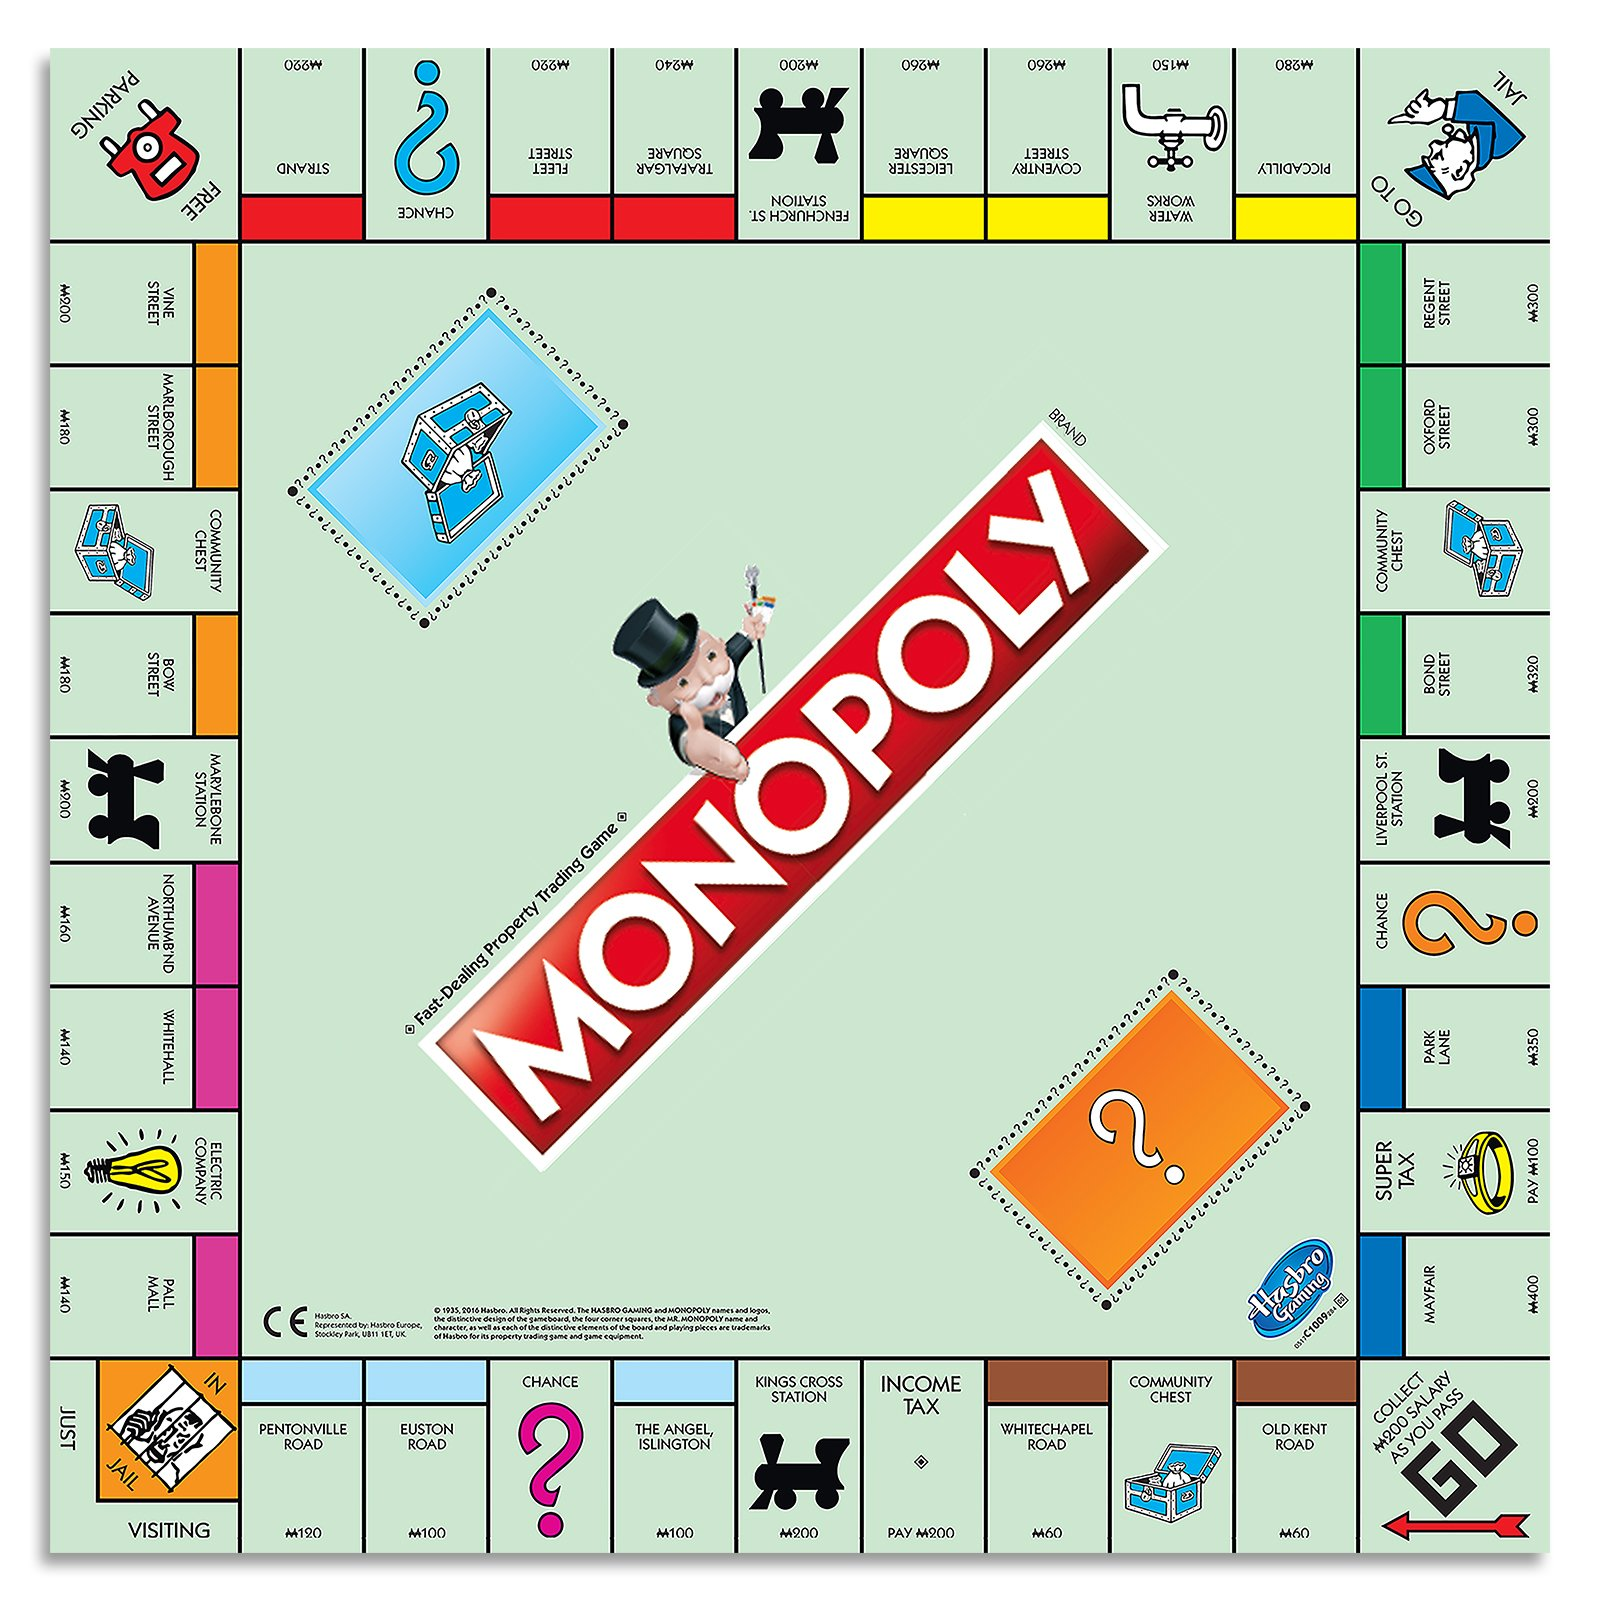
\includegraphics[width = \textwidth]{images/board.jpg}
\caption{The classic Monopoly board \cite{mon_board_image}}
\end{figure}

We will now describe each square with its associated action.
\begin{center} 
\begin{tabular}{|c|c|c|}
\hline
\textbf{Square index} & \textbf{Square name} & \textbf{Square action}\\
\hline 
1 & Start & Receive \$ 200\\
\hline
2 & Mediterranean Avenue & Property\\
\hline
3 & Community Chest & Grab a community chest card\\
\end{tabular}
\end{center}
\begin{thebibliography}{9}
\bibitem{mon_board_image} This is some information about the source
\end{thebibliography}

\end{document}